\chapter{Ověření Funkčnosti a vyměnění LED pásků}

Program i LED pásek mi fungoval tak, jak jsem přepokládala a tak jsem se se rozhodla vyměnint zkušební pevný LEDpásek, za původně předpokládaný ohebný. Udělala jsem to tak, jako předtím. Vzala jsem si tři obyčejné drátky a připájela je ke třem vstupním pinům co na pásku byli: Napájení, uzemění a řídící pin. Na druhou stranu drátů jsem přidala ((Takovou tu věc co musím zjistit jak se jmenuje)) a řídící pin jsem zase nechala na 21 pinu na ESP DevKit. 

%todo printscreen mobilu

Aby ale tento pásek fungoval, musela jsem v programu změnit proměnnou LED COUNT z 8 ledek na čtyři... protože ohebný LED pásek byl 
mnohem kratší než původní pásek testovací. 
%obrázky toho jak jsem připájela ohebný LED pásek
%todo Natočení videa a nahrání ho na internet!
%\begin{figure}[htbp]
%	\centering
%	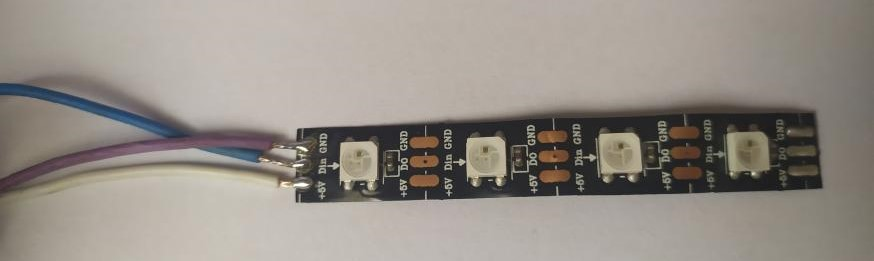
\includegraphics[width=0.7\textwidth]{img/4Led2.jpg}
%	\caption{Pásek se zapájenými dráty}
%	%	\label{fig:install-sdk-3}
%\end{figure}\chapter{Použité součástky}

V této kapitole budou představeny součástky, se kterými se v budoucnu použijeme

\section{ESP32 DevkitC}
%Co to je?
ESP32-DevKitC je malá programovatelná deska založená na ESP32 od společnosti Espressif. Vstupní a výstupní piny se nachází na obou stranách desky, což umožňuje uživateli připoji periferní zařízení jak pomocí propojovacích vodičů, tak připojením k nepájivému poli. Na desce se také nachází mikro-USB port který dovoluje  desku jedoduše napájet přímo z počítače, stejně jako nahrávat na desku soubory. 

\begin{figure}[htbp]
	\centering
	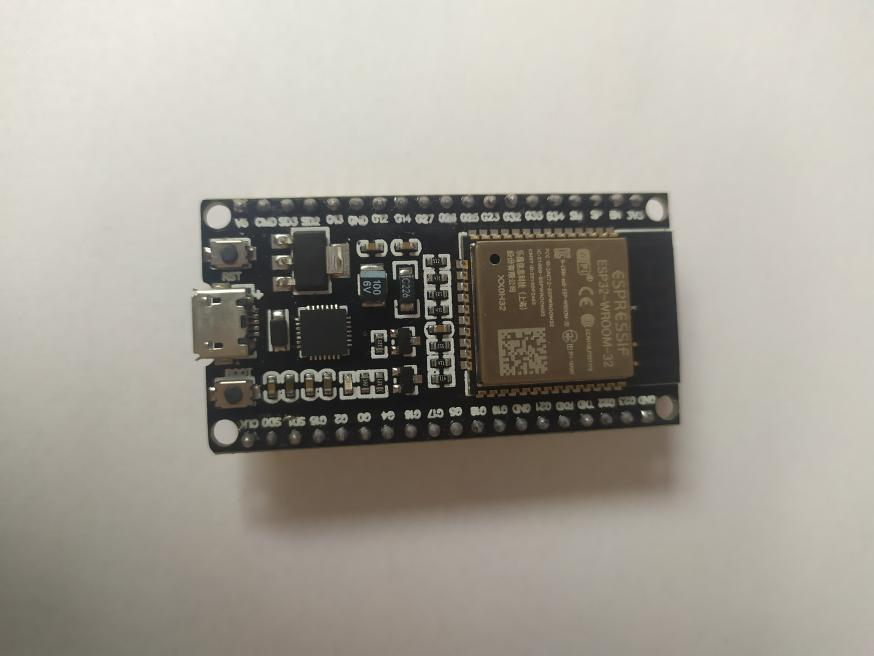
\includegraphics[width=0.7\textwidth]{img/ESPDevKit.jpg}
	\caption{ESPDevKit}
	%	\label{fig:install-sdk-3}
\end{figure}

%Co se s tím dá dělat
Deska je pompatibilní s Arduinem a často se v kombinaci zrovna s tímto typem součástek používá. Díky zabudovanému Wifi modulu je možné se na součástku napojit a používat jakékoliv zařízení pracující s Wifi, (například chytrý mobil), aby se k součástce napojilo a fungovalo jako dálkový ovladač, což jsem v praxi nejčastěji viděla už ke zvýše zmíněnému programování LED světel, ale prakticky se s ESP32 DevkitC dá dělat prakticky cokoliv: Použít ho jako procesor pro po domácku vyrobený alarm, nebo zaznamenávaše počasí. 


%Proč jsem si vybrala zrovna tuto součástku.
Já se ESP32 DevkitC rozhodla použít nejen proto, že v mém okolí mělo spoustu lidí s touto technoligií zkušenosti a mohli mi v případě nějakého problému jednoduše pomoct, ale hlavně kvůli dostupnosti a všestranému využití. Navíc Wifi modul na této desce se jednoduše dá využít pro dálkové ovládání ESP32 z mobilu což vyhovuje našim záměrům. Navíc rozměry desky ESP32 DevkitC(přibližně 5,5 cm na 3 cm) jsou vyhovující pro pozdější vybudování napájecí základny, která bude napájet a řídit LEDky schované v průchledném plastové květině.



\section{NeoPixel modul s 8 RGB LED WS2812}
%Co to je? Co se s tím dá dělat
Jedná se o pevný pásek s inteligentními LED diodami za sebou. Často využívá jako výstupní model pro Arduino a obsahuje 8 RGB LED diod typu WS2812, kterou lze najít i pod označením NeoPixel. Výhoda tohoto LED pásku je, že se dá řídit pomocí jednoho datového pinu a dvěma napájecími piny, což umožňuje kontrolér ve WS diodách. Tento modul se sice nehodí našemu původnímu záměru, který vyžaduje, ale Ledky byli na pásku ohebném, ale jako modul pro testování postačí.

\begin{figure}[htbp]
	\centering
	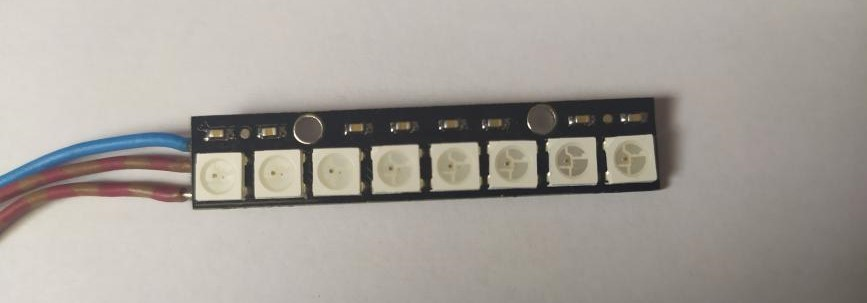
\includegraphics[width=0.7\textwidth]{img/NeoPixel2.jpg}
	\caption{NeoPixel}
	%	\label{fig:install-sdk-3}
\end{figure}

%Proč jsem si vybrala zrovna tuto součástku.
Tuto součástku jsem se rozhodla použít ze dvou důvodů. Ten první byl, že jsem neměla ještě úplně jistě vybraný finální ohebný led pásek, jaký bych chtěla použít. Ten druhý důvod byl stejně, jako v případě ESP, že kdyby nastaly při práci s tímto modulem nějaké problémy, tak jsem znala spoustu lidí, kteří by mi s případnými problémy dokázali pomoci. 


\section{Pásek ws2812 ohebný}
Po nějaké době práce s předchozím LED-páskem jsem si nakonec rozhodla vybrat skoro totožný pásek až na určitou maličkost, a to, aby byl Jednoduše ohebný a tvarovatelný. Pracuje a programuje se s ním stejně, jako s předchozím páskem, avšak, jelikož to více vyhovovalo záměru tak jsem tentokrát použila pásek se čtyřmi RGB LED diodami. 


\begin{figure}[htbp]
	\centering
	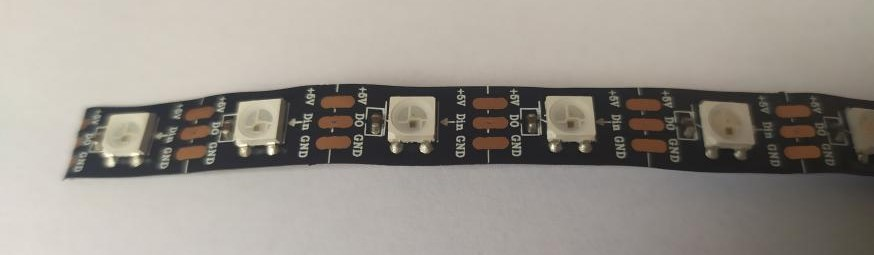
\includegraphics[width=0.7\textwidth]{img/OhebnyLedPasek2.jpg}
	\caption{{Pásek ws2812}
	%	\label{fig:install-sdk-3}
\end{figure}


\section{Pájení}

Proto, abych s těmito součástkami mohla dál pracovat, potřebovala jsem napojit Pevný LED NeoPixel pásek na ESPDevKit. Což jsem udělala tak, že jsem k Neopixel pásku připájela dráty na kontakty: napájení, uzemění a vstupní pin. Na tyto dráy jsem z druhé strany přidělala ((Ta černá koncovka která nevím jak se jmenuje)) a napojila jsem je z druhé strany na ESPDevKit. Jako vstupní pin jsem zvolila pin č. 21.  


%Otázky na učitele:
%Mám přidat obrázky? 
%Nevím jak pojmenávávat jednotlivé komponenty. Stačí to takhle? 

%Ostatní poznámky:
%Deska má tři druhy napájení, ale já budu využívat pouze napájení zkrz mikro-USB protože je to pro mě nejjednodušší. Stejně tak do toho budu posílat nahrané soubory z počítače
%Je potřeba vymyslet systém napájení
%Jak to funguje? Jaké je rozložení dané desky? 



%\lstinputlisting{priklady_c/blikani_LED1.cpp}
%\lstinputlisting{blikani_LED1.cpp}

\newpage